\documentclass[twoside]{book}

% Packages required by doxygen
\usepackage{fixltx2e}
\usepackage{calc}
\usepackage{doxygen}
\usepackage[export]{adjustbox} % also loads graphicx
\usepackage{graphicx}
\usepackage[utf8]{inputenc}
\usepackage{makeidx}
\usepackage{multicol}
\usepackage{multirow}
\PassOptionsToPackage{warn}{textcomp}
\usepackage{textcomp}
\usepackage[nointegrals]{wasysym}
\usepackage[table]{xcolor}

% Font selection
\usepackage[T1]{fontenc}
\usepackage[scaled=.90]{helvet}
\usepackage{courier}
\usepackage{amssymb}
\usepackage{sectsty}
\renewcommand{\familydefault}{\sfdefault}
\allsectionsfont{%
  \fontseries{bc}\selectfont%
  \color{darkgray}%
}
\renewcommand{\DoxyLabelFont}{%
  \fontseries{bc}\selectfont%
  \color{darkgray}%
}
\newcommand{\+}{\discretionary{\mbox{\scriptsize$\hookleftarrow$}}{}{}}

% Page & text layout
\usepackage{geometry}
\geometry{%
  a4paper,%
  top=2.5cm,%
  bottom=2.5cm,%
  left=2.5cm,%
  right=2.5cm%
}
\tolerance=750
\hfuzz=15pt
\hbadness=750
\setlength{\emergencystretch}{15pt}
\setlength{\parindent}{0cm}
\setlength{\parskip}{3ex plus 2ex minus 2ex}
\makeatletter
\renewcommand{\paragraph}{%
  \@startsection{paragraph}{4}{0ex}{-1.0ex}{1.0ex}{%
    \normalfont\normalsize\bfseries\SS@parafont%
  }%
}
\renewcommand{\subparagraph}{%
  \@startsection{subparagraph}{5}{0ex}{-1.0ex}{1.0ex}{%
    \normalfont\normalsize\bfseries\SS@subparafont%
  }%
}
\makeatother

% Headers & footers
\usepackage{fancyhdr}
\pagestyle{fancyplain}
\fancyhead[LE]{\fancyplain{}{\bfseries\thepage}}
\fancyhead[CE]{\fancyplain{}{}}
\fancyhead[RE]{\fancyplain{}{\bfseries\leftmark}}
\fancyhead[LO]{\fancyplain{}{\bfseries\rightmark}}
\fancyhead[CO]{\fancyplain{}{}}
\fancyhead[RO]{\fancyplain{}{\bfseries\thepage}}
\fancyfoot[LE]{\fancyplain{}{}}
\fancyfoot[CE]{\fancyplain{}{}}
\fancyfoot[RE]{\fancyplain{}{\bfseries\scriptsize Generated by Doxygen }}
\fancyfoot[LO]{\fancyplain{}{\bfseries\scriptsize Generated by Doxygen }}
\fancyfoot[CO]{\fancyplain{}{}}
\fancyfoot[RO]{\fancyplain{}{}}
\renewcommand{\footrulewidth}{0.4pt}
\renewcommand{\chaptermark}[1]{%
  \markboth{#1}{}%
}
\renewcommand{\sectionmark}[1]{%
  \markright{\thesection\ #1}%
}

% Indices & bibliography
\usepackage{natbib}
\usepackage[titles]{tocloft}
\setcounter{tocdepth}{3}
\setcounter{secnumdepth}{5}
\makeindex

% Hyperlinks (required, but should be loaded last)
\usepackage{ifpdf}
\ifpdf
  \usepackage[pdftex,pagebackref=true]{hyperref}
\else
  \usepackage[ps2pdf,pagebackref=true]{hyperref}
\fi
\hypersetup{%
  colorlinks=true,%
  linkcolor=blue,%
  citecolor=blue,%
  unicode%
}

% Custom commands
\newcommand{\clearemptydoublepage}{%
  \newpage{\pagestyle{empty}\cleardoublepage}%
}

\usepackage{caption}
\captionsetup{labelsep=space,justification=centering,font={bf},singlelinecheck=off,skip=4pt,position=top}

%===== C O N T E N T S =====

\begin{document}

% Titlepage & ToC
\hypersetup{pageanchor=false,
             bookmarksnumbered=true,
             pdfencoding=unicode
            }
\pagenumbering{roman}
\begin{titlepage}
\vspace*{7cm}
\begin{center}%
{\Large Race\+Control \\[1ex]\large 1.\+0 }\\
\vspace*{1cm}
{\large Generated by Doxygen 1.8.11}\\
\end{center}
\end{titlepage}
\clearemptydoublepage
\tableofcontents
\clearemptydoublepage
\pagenumbering{arabic}
\hypersetup{pageanchor=true}

%--- Begin generated contents ---
\chapter{About}
\label{md_README}
\hypertarget{md_README}{}
If you\textquotesingle{}ve ever had to operate any vehicle carrying data on the C\+AN bus, there\textquotesingle{}s a fair chance that you have been forced to use closed source, limited capability tools. This is my B\+Sc project, maybe it can serve as the basis for something else, maybe you\textquotesingle{}re just interested. Enjoy.

todo\+: licensing

\section*{Install }

When it\textquotesingle{}s done\+: {\ttfamily python setup.\+py install}

Right now, it\textquotesingle{}s still a work in progress. 
\chapter{Hierarchical Index}
\section{Class Hierarchy}
This inheritance list is sorted roughly, but not completely, alphabetically\+:\begin{DoxyCompactList}
\item \contentsline{section}{racecontrol.\+cancom.\+C\+A\+N\+Com}{\pageref{classracecontrol_1_1cancom_1_1CANCom}}{}
\item Datagram\+Request\+Handler\begin{DoxyCompactList}
\item \contentsline{section}{racecontrol.\+netcom.\+Net\+Com\+Request\+Handler}{\pageref{classracecontrol_1_1netcom_1_1NetComRequestHandler}}{}
\end{DoxyCompactList}
\item \contentsline{section}{racecontrol.\+netcom.\+Dispatcher}{\pageref{classracecontrol_1_1netcom_1_1Dispatcher}}{}
\item \contentsline{section}{racecontrol.\+webcom.\+G\+U\+I\+Com}{\pageref{classracecontrol_1_1webcom_1_1GUICom}}{}
\item Listener\begin{DoxyCompactList}
\item \contentsline{section}{racecontrol.\+logcom.\+C\+S\+V\+Logger}{\pageref{classracecontrol_1_1logcom_1_1CSVLogger}}{}
\end{DoxyCompactList}
\item \contentsline{section}{racecontrol.\+logcom.\+Log\+Com}{\pageref{classracecontrol_1_1logcom_1_1LogCom}}{}
\item \contentsline{section}{racecontrol.\+netcom.\+Net\+Com}{\pageref{classracecontrol_1_1netcom_1_1NetCom}}{}
\item \contentsline{section}{racecontrol.\+netcom.\+Node}{\pageref{classracecontrol_1_1netcom_1_1Node}}{}
\item U\+D\+P\+Server\begin{DoxyCompactList}
\item \contentsline{section}{racecontrol.\+netcom.\+Net\+Com\+Server}{\pageref{classracecontrol_1_1netcom_1_1NetComServer}}{}
\end{DoxyCompactList}
\end{DoxyCompactList}

\chapter{Class Index}
\section{Class List}
Here are the classes, structs, unions and interfaces with brief descriptions\+:\begin{DoxyCompactList}
\item\contentsline{section}{\hyperlink{classracecontrol_1_1cancom_1_1CANCom}{racecontrol.\+cancom.\+C\+A\+N\+Com} }{\pageref{classracecontrol_1_1cancom_1_1CANCom}}{}
\item\contentsline{section}{\hyperlink{classracecontrol_1_1logcom_1_1CSVLogger}{racecontrol.\+logcom.\+C\+S\+V\+Logger} }{\pageref{classracecontrol_1_1logcom_1_1CSVLogger}}{}
\item\contentsline{section}{\hyperlink{classracecontrol_1_1netcom_1_1Dispatcher}{racecontrol.\+netcom.\+Dispatcher} }{\pageref{classracecontrol_1_1netcom_1_1Dispatcher}}{}
\item\contentsline{section}{\hyperlink{classracecontrol_1_1webcom_1_1GUICom}{racecontrol.\+webcom.\+G\+U\+I\+Com} }{\pageref{classracecontrol_1_1webcom_1_1GUICom}}{}
\item\contentsline{section}{\hyperlink{classracecontrol_1_1logcom_1_1LogCom}{racecontrol.\+logcom.\+Log\+Com} }{\pageref{classracecontrol_1_1logcom_1_1LogCom}}{}
\item\contentsline{section}{\hyperlink{classracecontrol_1_1netcom_1_1NetCom}{racecontrol.\+netcom.\+Net\+Com} }{\pageref{classracecontrol_1_1netcom_1_1NetCom}}{}
\item\contentsline{section}{\hyperlink{classracecontrol_1_1netcom_1_1NetComRequestHandler}{racecontrol.\+netcom.\+Net\+Com\+Request\+Handler} }{\pageref{classracecontrol_1_1netcom_1_1NetComRequestHandler}}{}
\item\contentsline{section}{\hyperlink{classracecontrol_1_1netcom_1_1NetComServer}{racecontrol.\+netcom.\+Net\+Com\+Server} }{\pageref{classracecontrol_1_1netcom_1_1NetComServer}}{}
\item\contentsline{section}{\hyperlink{classracecontrol_1_1netcom_1_1Node}{racecontrol.\+netcom.\+Node} }{\pageref{classracecontrol_1_1netcom_1_1Node}}{}
\end{DoxyCompactList}

\chapter{Class Documentation}
\hypertarget{classracecontrol_1_1cancom_1_1CANCom}{}\section{racecontrol.\+cancom.\+C\+A\+N\+Com Class Reference}
\label{classracecontrol_1_1cancom_1_1CANCom}\index{racecontrol.\+cancom.\+C\+A\+N\+Com@{racecontrol.\+cancom.\+C\+A\+N\+Com}}
\subsection*{Public Member Functions}
\begin{DoxyCompactItemize}
\item 
def {\bfseries \+\_\+\+\_\+init\+\_\+\+\_\+} (self, blacklist, interface=C\+A\+N\+\_\+\+I\+F\+A\+CE, listeners=\mbox{[}$\,$\mbox{]})\hypertarget{classracecontrol_1_1cancom_1_1CANCom_ab985a1ec22be9cf57bccec3e400a1383}{}\label{classracecontrol_1_1cancom_1_1CANCom_ab985a1ec22be9cf57bccec3e400a1383}

\item 
def \hyperlink{classracecontrol_1_1cancom_1_1CANCom_a17217b9206b06bfb080a34df26bf3e50}{add\+\_\+listener} (self, listener)
\item 
def \hyperlink{classracecontrol_1_1cancom_1_1CANCom_ac7aa4f352f75d0e1581323d2c8fb0d74}{run\+\_\+notifier} (self, timeout=None)
\item 
def \hyperlink{classracecontrol_1_1cancom_1_1CANCom_a6433c22844fea3f3f65f3103528c732c}{stop\+\_\+notifier} (self)
\item 
def \hyperlink{classracecontrol_1_1cancom_1_1CANCom_a909c7508693465607a71003014a14ffc}{operate} (self)
\end{DoxyCompactItemize}
\subsection*{Public Attributes}
\begin{DoxyCompactItemize}
\item 
{\bfseries blacklist}\hypertarget{classracecontrol_1_1cancom_1_1CANCom_a18b61f0fb38913869153e6d9d29722e5}{}\label{classracecontrol_1_1cancom_1_1CANCom_a18b61f0fb38913869153e6d9d29722e5}

\item 
{\bfseries bus}\hypertarget{classracecontrol_1_1cancom_1_1CANCom_a0d02fccc3ae1db96edf0ab37a63642ea}{}\label{classracecontrol_1_1cancom_1_1CANCom_a0d02fccc3ae1db96edf0ab37a63642ea}

\item 
{\bfseries interface}\hypertarget{classracecontrol_1_1cancom_1_1CANCom_a57730a29aa159916aaba10d8bef3e2f4}{}\label{classracecontrol_1_1cancom_1_1CANCom_a57730a29aa159916aaba10d8bef3e2f4}

\item 
{\bfseries listeners}\hypertarget{classracecontrol_1_1cancom_1_1CANCom_ab5609d47b9144f9d53a71273d03deec6}{}\label{classracecontrol_1_1cancom_1_1CANCom_ab5609d47b9144f9d53a71273d03deec6}

\item 
{\bfseries buffer}\hypertarget{classracecontrol_1_1cancom_1_1CANCom_ab2666668b9d321a5659448b044c8b607}{}\label{classracecontrol_1_1cancom_1_1CANCom_ab2666668b9d321a5659448b044c8b607}

\item 
{\bfseries notifier}\hypertarget{classracecontrol_1_1cancom_1_1CANCom_a13c3f606fc3ee8bafd78b2694d3133c4}{}\label{classracecontrol_1_1cancom_1_1CANCom_a13c3f606fc3ee8bafd78b2694d3133c4}

\item 
{\bfseries running}\hypertarget{classracecontrol_1_1cancom_1_1CANCom_ad505d0df53d256b1d534952b07e10f63}{}\label{classracecontrol_1_1cancom_1_1CANCom_ad505d0df53d256b1d534952b07e10f63}

\end{DoxyCompactItemize}


\subsection{Detailed Description}
\begin{DoxyVerb}CANCom class for establishing the CAN bus connection and
sending/receiving on it.

The CANCom class, when instantiated, establishes the CAN bus connection and
starts a thread to transmit CAN data received from other application
sources. It also instantiates a can.Notifier object which is itself a
threaded listener on the CAN bus and connects it to the listeners it knows.
\end{DoxyVerb}
 

\subsection{Member Function Documentation}
\index{racecontrol\+::cancom\+::\+C\+A\+N\+Com@{racecontrol\+::cancom\+::\+C\+A\+N\+Com}!add\+\_\+listener@{add\+\_\+listener}}
\index{add\+\_\+listener@{add\+\_\+listener}!racecontrol\+::cancom\+::\+C\+A\+N\+Com@{racecontrol\+::cancom\+::\+C\+A\+N\+Com}}
\subsubsection[{\texorpdfstring{add\+\_\+listener(self, listener)}{add_listener(self, listener)}}]{\setlength{\rightskip}{0pt plus 5cm}def racecontrol.\+cancom.\+C\+A\+N\+Com.\+add\+\_\+listener (
\begin{DoxyParamCaption}
\item[{}]{self, }
\item[{}]{listener}
\end{DoxyParamCaption}
)}\hypertarget{classracecontrol_1_1cancom_1_1CANCom_a17217b9206b06bfb080a34df26bf3e50}{}\label{classracecontrol_1_1cancom_1_1CANCom_a17217b9206b06bfb080a34df26bf3e50}
\begin{DoxyVerb}Method to add a listener to a CANCom object. All listeners in a CANCom
object are notified when a message is read from the bus.
\end{DoxyVerb}
 \index{racecontrol\+::cancom\+::\+C\+A\+N\+Com@{racecontrol\+::cancom\+::\+C\+A\+N\+Com}!operate@{operate}}
\index{operate@{operate}!racecontrol\+::cancom\+::\+C\+A\+N\+Com@{racecontrol\+::cancom\+::\+C\+A\+N\+Com}}
\subsubsection[{\texorpdfstring{operate(self)}{operate(self)}}]{\setlength{\rightskip}{0pt plus 5cm}def racecontrol.\+cancom.\+C\+A\+N\+Com.\+operate (
\begin{DoxyParamCaption}
\item[{}]{self}
\end{DoxyParamCaption}
)}\hypertarget{classracecontrol_1_1cancom_1_1CANCom_a909c7508693465607a71003014a14ffc}{}\label{classracecontrol_1_1cancom_1_1CANCom_a909c7508693465607a71003014a14ffc}
\begin{DoxyVerb}Method which is the target of the thread. It listens to the object's
message buffer for messages from the other application members and, if
there is a message, sends it to the CAN bus after filtering it with the
blacklist.
\end{DoxyVerb}
 \index{racecontrol\+::cancom\+::\+C\+A\+N\+Com@{racecontrol\+::cancom\+::\+C\+A\+N\+Com}!run\+\_\+notifier@{run\+\_\+notifier}}
\index{run\+\_\+notifier@{run\+\_\+notifier}!racecontrol\+::cancom\+::\+C\+A\+N\+Com@{racecontrol\+::cancom\+::\+C\+A\+N\+Com}}
\subsubsection[{\texorpdfstring{run\+\_\+notifier(self, timeout=\+None)}{run_notifier(self, timeout=None)}}]{\setlength{\rightskip}{0pt plus 5cm}def racecontrol.\+cancom.\+C\+A\+N\+Com.\+run\+\_\+notifier (
\begin{DoxyParamCaption}
\item[{}]{self, }
\item[{}]{timeout = {\ttfamily None}}
\end{DoxyParamCaption}
)}\hypertarget{classracecontrol_1_1cancom_1_1CANCom_ac7aa4f352f75d0e1581323d2c8fb0d74}{}\label{classracecontrol_1_1cancom_1_1CANCom_ac7aa4f352f75d0e1581323d2c8fb0d74}
\begin{DoxyVerb}Method to create a new Notifier on the CANCom object's bus. Returns an
instantiated can.Notifier object. Used to create a new notifier object
whenever a listener is added.
\end{DoxyVerb}
 \index{racecontrol\+::cancom\+::\+C\+A\+N\+Com@{racecontrol\+::cancom\+::\+C\+A\+N\+Com}!stop\+\_\+notifier@{stop\+\_\+notifier}}
\index{stop\+\_\+notifier@{stop\+\_\+notifier}!racecontrol\+::cancom\+::\+C\+A\+N\+Com@{racecontrol\+::cancom\+::\+C\+A\+N\+Com}}
\subsubsection[{\texorpdfstring{stop\+\_\+notifier(self)}{stop_notifier(self)}}]{\setlength{\rightskip}{0pt plus 5cm}def racecontrol.\+cancom.\+C\+A\+N\+Com.\+stop\+\_\+notifier (
\begin{DoxyParamCaption}
\item[{}]{self}
\end{DoxyParamCaption}
)}\hypertarget{classracecontrol_1_1cancom_1_1CANCom_a6433c22844fea3f3f65f3103528c732c}{}\label{classracecontrol_1_1cancom_1_1CANCom_a6433c22844fea3f3f65f3103528c732c}
\begin{DoxyVerb}Method to stop the current notifier. Used whenever a listener is added
to stop the old notifier so the thread won't become zombied in the
interpreter.
\end{DoxyVerb}
 

The documentation for this class was generated from the following file\+:\begin{DoxyCompactItemize}
\item 
racecontrol/cancom.\+py\end{DoxyCompactItemize}

\section{racecontrol.\+logcom.\+C\+S\+V\+Logger Class Reference}
\label{classracecontrol_1_1logcom_1_1CSVLogger}\index{racecontrol.\+logcom.\+C\+S\+V\+Logger@{racecontrol.\+logcom.\+C\+S\+V\+Logger}}
Inheritance diagram for racecontrol.\+logcom.\+C\+S\+V\+Logger\+:\begin{figure}[H]
\begin{center}
\leavevmode
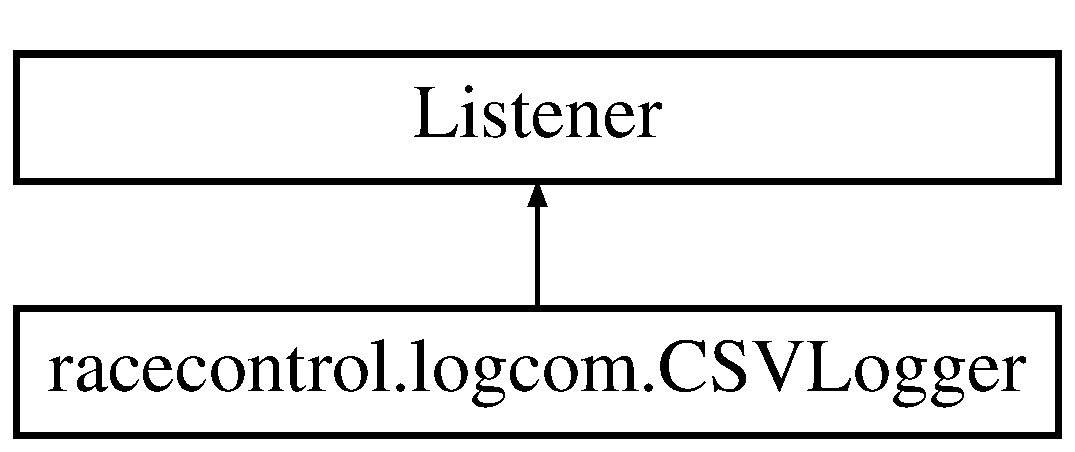
\includegraphics[height=2.000000cm]{classracecontrol_1_1logcom_1_1CSVLogger}
\end{center}
\end{figure}
\subsection*{Public Member Functions}
\begin{DoxyCompactItemize}
\item 
def {\bfseries \+\_\+\+\_\+init\+\_\+\+\_\+} (self, device, interface, filename)\label{classracecontrol_1_1logcom_1_1CSVLogger_a9c2aeb6deff0ce6f9543c8f56b02d684}

\item 
def {\bf on\+\_\+message\+\_\+received} (self, msg)
\item 
def {\bf \+\_\+\+\_\+del\+\_\+\+\_\+} (self)
\end{DoxyCompactItemize}
\subsection*{Public Attributes}
\begin{DoxyCompactItemize}
\item 
{\bfseries device}\label{classracecontrol_1_1logcom_1_1CSVLogger_a95f52b7ee93b7cffe3e90573f471445d}

\item 
{\bfseries interface}\label{classracecontrol_1_1logcom_1_1CSVLogger_a7699efcb2269db009a16a1d0480d69a6}

\item 
{\bfseries flushstamp}\label{classracecontrol_1_1logcom_1_1CSVLogger_a30078c3a214fefa381fcfccfbe4a3681}

\item 
{\bfseries filename}\label{classracecontrol_1_1logcom_1_1CSVLogger_a1224e8bf10827b6a7be2cc8ff4d60b35}

\item 
{\bfseries file}\label{classracecontrol_1_1logcom_1_1CSVLogger_a7673704993c47cf5adc04ff49512c1f0}

\end{DoxyCompactItemize}


\subsection{Detailed Description}
\begin{DoxyVerb}Implements the can.Listener interface and writes messages in RaceControl
CSV files.

This class implements the can.Listener interface, which makes it callable
from objects of the can.Notifier class with can.Message objects. On
instantiation, it sets a timeout counter for flushing to file in case the
file is downloaded intermittently and opens a file with user defined
filename.
\end{DoxyVerb}
 

\subsection{Constructor \& Destructor Documentation}
\index{racecontrol\+::logcom\+::\+C\+S\+V\+Logger@{racecontrol\+::logcom\+::\+C\+S\+V\+Logger}!\+\_\+\+\_\+del\+\_\+\+\_\+@{\+\_\+\+\_\+del\+\_\+\+\_\+}}
\index{\+\_\+\+\_\+del\+\_\+\+\_\+@{\+\_\+\+\_\+del\+\_\+\+\_\+}!racecontrol\+::logcom\+::\+C\+S\+V\+Logger@{racecontrol\+::logcom\+::\+C\+S\+V\+Logger}}
\subsubsection[{\+\_\+\+\_\+del\+\_\+\+\_\+(self)}]{\setlength{\rightskip}{0pt plus 5cm}def racecontrol.\+logcom.\+C\+S\+V\+Logger.\+\_\+\+\_\+del\+\_\+\+\_\+ (
\begin{DoxyParamCaption}
\item[{}]{self}
\end{DoxyParamCaption}
)}\label{classracecontrol_1_1logcom_1_1CSVLogger_a096f839011bd342fdf239a767d07f384}
\begin{DoxyVerb}Standard method called when the interpreter's garbage collector picks
the object up. Since data is flushed via timeout and the garbage
collector should close the open file object eventually as well, this is
not technically necessary, but added for safety.
\end{DoxyVerb}
 

\subsection{Member Function Documentation}
\index{racecontrol\+::logcom\+::\+C\+S\+V\+Logger@{racecontrol\+::logcom\+::\+C\+S\+V\+Logger}!on\+\_\+message\+\_\+received@{on\+\_\+message\+\_\+received}}
\index{on\+\_\+message\+\_\+received@{on\+\_\+message\+\_\+received}!racecontrol\+::logcom\+::\+C\+S\+V\+Logger@{racecontrol\+::logcom\+::\+C\+S\+V\+Logger}}
\subsubsection[{on\+\_\+message\+\_\+received(self, msg)}]{\setlength{\rightskip}{0pt plus 5cm}def racecontrol.\+logcom.\+C\+S\+V\+Logger.\+on\+\_\+message\+\_\+received (
\begin{DoxyParamCaption}
\item[{}]{self, }
\item[{}]{msg}
\end{DoxyParamCaption}
)}\label{classracecontrol_1_1logcom_1_1CSVLogger_aa707d38f31fff151568318af99cc4235}
\begin{DoxyVerb}Implements can.Listener's on_message_received method. Then proceeds to
join all elements in the can.Message object it gets passed into a
RaceControl CSV string and writes the string to file.
\end{DoxyVerb}
 

The documentation for this class was generated from the following file\+:\begin{DoxyCompactItemize}
\item 
racecontrol/logcom.\+py\end{DoxyCompactItemize}

\section{racecontrol.\+netcom.\+Dispatcher Class Reference}
\label{classracecontrol_1_1netcom_1_1Dispatcher}\index{racecontrol.\+netcom.\+Dispatcher@{racecontrol.\+netcom.\+Dispatcher}}
\subsection*{Public Member Functions}
\begin{DoxyCompactItemize}
\item 
def {\bfseries \+\_\+\+\_\+init\+\_\+\+\_\+} (self, netcom, prioritylist, port=D\+\_\+\+P\+O\+RT, timeout=100)\label{classracecontrol_1_1netcom_1_1Dispatcher_a40d53ebebdec4c628392f666ff14a4f4}

\item 
def {\bf priorityfilter} (self, msg)
\item 
def {\bf dispatch} (self, payload)
\item 
def {\bf operate} (self)
\end{DoxyCompactItemize}
\subsection*{Public Attributes}
\begin{DoxyCompactItemize}
\item 
{\bfseries buffer}\label{classracecontrol_1_1netcom_1_1Dispatcher_a1b53b2fd4b2dbde0e3cc31a5416fbd2e}

\item 
{\bfseries prioritylist}\label{classracecontrol_1_1netcom_1_1Dispatcher_a5cafa237d7e25d70d330cc7a12f6c93a}

\item 
{\bfseries priority\+\_\+set}\label{classracecontrol_1_1netcom_1_1Dispatcher_a71685a4d695523d4485bda704f53ede9}

\item 
{\bfseries netcom}\label{classracecontrol_1_1netcom_1_1Dispatcher_a7880baacf7b0928435ac9fe2088ac0ed}

\item 
{\bfseries port}\label{classracecontrol_1_1netcom_1_1Dispatcher_a93f7c9e98ee6b191761b7f04ddf26261}

\item 
{\bfseries sock}\label{classracecontrol_1_1netcom_1_1Dispatcher_ac347291950368776556f36686d7c54d1}

\item 
{\bfseries timeout}\label{classracecontrol_1_1netcom_1_1Dispatcher_a0f007223f86688ce9fd62b8d44c428bc}

\item 
{\bfseries trigger}\label{classracecontrol_1_1netcom_1_1Dispatcher_a47286311bec7ca31f504296cc434866e}

\item 
{\bfseries running}\label{classracecontrol_1_1netcom_1_1Dispatcher_a91cf54434cc2b6fe4b66d5d0680e2229}

\end{DoxyCompactItemize}


\subsection{Detailed Description}
\begin{DoxyVerb}Handles dispatching can.Message objects over the UDP connection.

The Dispatcher object is in charge of sending CAN messages over the UDP
connection. It offers a priority_set variable which can be used to set
priority mode. It also holds a can.BufferedReader receiving connections
from other RaceControl objects. It starts a thread to operate the
connection using the operate() method.
\end{DoxyVerb}
 

\subsection{Member Function Documentation}
\index{racecontrol\+::netcom\+::\+Dispatcher@{racecontrol\+::netcom\+::\+Dispatcher}!dispatch@{dispatch}}
\index{dispatch@{dispatch}!racecontrol\+::netcom\+::\+Dispatcher@{racecontrol\+::netcom\+::\+Dispatcher}}
\subsubsection[{dispatch(self, payload)}]{\setlength{\rightskip}{0pt plus 5cm}def racecontrol.\+netcom.\+Dispatcher.\+dispatch (
\begin{DoxyParamCaption}
\item[{}]{self, }
\item[{}]{payload}
\end{DoxyParamCaption}
)}\label{classracecontrol_1_1netcom_1_1Dispatcher_a1972a5b40129984301084ff41eab5824}
\begin{DoxyVerb}Dispatches bytearrays to all nodes known to the NetCom object this
Dispatcher object is connected to.
\end{DoxyVerb}
 \index{racecontrol\+::netcom\+::\+Dispatcher@{racecontrol\+::netcom\+::\+Dispatcher}!operate@{operate}}
\index{operate@{operate}!racecontrol\+::netcom\+::\+Dispatcher@{racecontrol\+::netcom\+::\+Dispatcher}}
\subsubsection[{operate(self)}]{\setlength{\rightskip}{0pt plus 5cm}def racecontrol.\+netcom.\+Dispatcher.\+operate (
\begin{DoxyParamCaption}
\item[{}]{self}
\end{DoxyParamCaption}
)}\label{classracecontrol_1_1netcom_1_1Dispatcher_ae54f350204273958e80248a56943fc0c}
\begin{DoxyVerb}Target for the thread. Reads messages from the message buffer and puts
them into the priority filter. If they come back and are not empty, the
operate() method puts them into the dispatch() method. Furthermore, it
dispatches a register protocol messages to all nodes as a keepalive
message every few seconds in case there are no CAN messages to be
transmitted.
\end{DoxyVerb}
 \index{racecontrol\+::netcom\+::\+Dispatcher@{racecontrol\+::netcom\+::\+Dispatcher}!priorityfilter@{priorityfilter}}
\index{priorityfilter@{priorityfilter}!racecontrol\+::netcom\+::\+Dispatcher@{racecontrol\+::netcom\+::\+Dispatcher}}
\subsubsection[{priorityfilter(self, msg)}]{\setlength{\rightskip}{0pt plus 5cm}def racecontrol.\+netcom.\+Dispatcher.\+priorityfilter (
\begin{DoxyParamCaption}
\item[{}]{self, }
\item[{}]{msg}
\end{DoxyParamCaption}
)}\label{classracecontrol_1_1netcom_1_1Dispatcher_a01b0f08e2145db578fe74208d5e34d9e}
\begin{DoxyVerb}If priority_set is set to True, this method filters messages through
the priority list and returns None if the message is not in the list.
If priority_set is set to False, it returns the msg instantly.
\end{DoxyVerb}
 

The documentation for this class was generated from the following file\+:\begin{DoxyCompactItemize}
\item 
racecontrol/netcom.\+py\end{DoxyCompactItemize}

\section{racecontrol.\+webcom.\+G\+U\+I\+Com Class Reference}
\label{classracecontrol_1_1webcom_1_1GUICom}\index{racecontrol.\+webcom.\+G\+U\+I\+Com@{racecontrol.\+webcom.\+G\+U\+I\+Com}}
\subsection*{Public Member Functions}
\begin{DoxyCompactItemize}
\item 
def {\bfseries \+\_\+\+\_\+init\+\_\+\+\_\+} (self, queue, msgfilter)\label{classracecontrol_1_1webcom_1_1GUICom_a06515a6004ff7f8554ea65483de9e684}

\end{DoxyCompactItemize}
\subsection*{Public Attributes}
\begin{DoxyCompactItemize}
\item 
{\bfseries queue}\label{classracecontrol_1_1webcom_1_1GUICom_aaee4be625caecf5e88a86c69b9672e8a}

\item 
{\bfseries msgfilter}\label{classracecontrol_1_1webcom_1_1GUICom_a9a7fb7d0154519fb4b4f9c50f206cb9c}

\item 
{\bfseries buffer}\label{classracecontrol_1_1webcom_1_1GUICom_a5cef744c84d93e37ef0d6726df5b7595}

\item 
{\bfseries permsg}\label{classracecontrol_1_1webcom_1_1GUICom_a1e1dadd40a811d3f91290cf827f92ec9}

\end{DoxyCompactItemize}


\subsection{Detailed Description}
\begin{DoxyVerb}Gets can.Message objects and parses them through the msgfilter necessary
to create web interface suited CSV data.

The GUICom class has a threadsafe and processsafe queue it pushes the
generated message to and a can.BufferedReader object which is notified by
other RaceControl objects with can.Message objects. It starts a thread
which runs the web interface data generator.
\end{DoxyVerb}
 

The documentation for this class was generated from the following file\+:\begin{DoxyCompactItemize}
\item 
racecontrol/webcom.\+py\end{DoxyCompactItemize}

\section{racecontrol.\+logcom.\+Log\+Com Class Reference}
\label{classracecontrol_1_1logcom_1_1LogCom}\index{racecontrol.\+logcom.\+Log\+Com@{racecontrol.\+logcom.\+Log\+Com}}
\subsection*{Public Member Functions}
\begin{DoxyCompactItemize}
\item 
def {\bfseries \+\_\+\+\_\+init\+\_\+\+\_\+} (self, logdir=L\+O\+G\+D\+IR, fileformat=F\+I\+L\+E\+F\+O\+R\+M\+AT)\label{classracecontrol_1_1logcom_1_1LogCom_a1b7430f202da41f27eb9d471fecd4cb4}

\item 
def {\bf loggers} (self)
\end{DoxyCompactItemize}
\subsection*{Public Attributes}
\begin{DoxyCompactItemize}
\item 
{\bfseries device}\label{classracecontrol_1_1logcom_1_1LogCom_ae44ae38fb3b18b6cdd7892d771029f86}

\item 
{\bfseries interface}\label{classracecontrol_1_1logcom_1_1LogCom_a29decd0250cfc7548f95b0855b1d1331}

\item 
{\bfseries logdir}\label{classracecontrol_1_1logcom_1_1LogCom_af2d649bd23fb2593cb5043afcd227cc9}

\item 
{\bfseries fileformat}\label{classracecontrol_1_1logcom_1_1LogCom_ada32b5a1e4dbbf4ddd403609146b5524}

\item 
{\bfseries csv\+\_\+logger}\label{classracecontrol_1_1logcom_1_1LogCom_a5ab3a32ec26a4c6be022d3efda81f396}

\end{DoxyCompactItemize}


\subsection{Detailed Description}
\begin{DoxyVerb}Instatiates CSVLogger objects with user defined timestamps as filename
patterns.

The LogCom class, when instantiated, parses the input strings containing
the timestamping patterns for the logging filename through the arrow
library, which provides beautifully formatted strings with timestamps. It
then creates a CSVLogger object it uses to log messages to a file.
\end{DoxyVerb}
 

\subsection{Member Function Documentation}
\index{racecontrol\+::logcom\+::\+Log\+Com@{racecontrol\+::logcom\+::\+Log\+Com}!loggers@{loggers}}
\index{loggers@{loggers}!racecontrol\+::logcom\+::\+Log\+Com@{racecontrol\+::logcom\+::\+Log\+Com}}
\subsubsection[{loggers(self)}]{\setlength{\rightskip}{0pt plus 5cm}def racecontrol.\+logcom.\+Log\+Com.\+loggers (
\begin{DoxyParamCaption}
\item[{}]{self}
\end{DoxyParamCaption}
)}\label{classracecontrol_1_1logcom_1_1LogCom_a5cf7d193b6c1f32ebc5a5c6ea47cd76f}
\begin{DoxyVerb}Function which returns the current loggers owned by the LogCom object.
The main function of the RaceControl package loops through this and
distributes the objects to the other application members. Loggers have
to implement the can.Listener interface for this to work.
\end{DoxyVerb}
 

The documentation for this class was generated from the following file\+:\begin{DoxyCompactItemize}
\item 
racecontrol/logcom.\+py\end{DoxyCompactItemize}

\section{racecontrol.\+netcom.\+Net\+Com Class Reference}
\label{classracecontrol_1_1netcom_1_1NetCom}\index{racecontrol.\+netcom.\+Net\+Com@{racecontrol.\+netcom.\+Net\+Com}}
\subsection*{Public Member Functions}
\begin{DoxyCompactItemize}
\item 
def {\bfseries \+\_\+\+\_\+init\+\_\+\+\_\+} (self, prioritylist, ip=\textquotesingle{}192.\+168.\+11.\+26\textquotesingle{}, udpport=D\+\_\+\+P\+O\+RT, listeners=[$\,$], node\+\_\+ips=N\+O\+D\+ES)\label{classracecontrol_1_1netcom_1_1NetCom_a3decf896d9d62b9a3fd06dffef2b3fe5}

\item 
def {\bf add\+\_\+listener} (self, listener)
\item 
def {\bf notify} (self, msg)
\item 
def {\bf add\+\_\+node} (self, node\+\_\+ip, last\+\_\+msg=None)
\item 
def {\bf ip\+\_\+list} (self)
\item 
def {\bf check\+\_\+nodes} (self)
\end{DoxyCompactItemize}
\subsection*{Public Attributes}
\begin{DoxyCompactItemize}
\item 
{\bfseries ip}\label{classracecontrol_1_1netcom_1_1NetCom_a655c019f1760dc2aeac17059daa9003e}

\item 
{\bfseries udpport}\label{classracecontrol_1_1netcom_1_1NetCom_ab1de996cc0fbaa07ff432eb49111220a}

\item 
{\bfseries listeners}\label{classracecontrol_1_1netcom_1_1NetCom_af65e46142c5376a0e20642b064daf791}

\item 
{\bfseries nodes}\label{classracecontrol_1_1netcom_1_1NetCom_ab7425c0021edb0748e364bed18b0bdbd}

\item 
{\bfseries dispatcher}\label{classracecontrol_1_1netcom_1_1NetCom_a7220c84e9eaf348fe1e11be8d29e2c7e}

\item 
{\bfseries running}\label{classracecontrol_1_1netcom_1_1NetCom_aec956fd7586eccce58253004e0e77f83}

\end{DoxyCompactItemize}


\subsection{Detailed Description}
\begin{DoxyVerb}Handles UDP network communication.

The NetCom class instantiates Node objects for all node IPs give in the
config file and registers them. It then broadcasts the protocol message
used to register with other nodes and starts threads for both the UDP
server and the watchdog. The watchdog takes care of checking node activity
and remove inactive nodes from the NetCom object's register.
\end{DoxyVerb}
 

\subsection{Member Function Documentation}
\index{racecontrol\+::netcom\+::\+Net\+Com@{racecontrol\+::netcom\+::\+Net\+Com}!add\+\_\+listener@{add\+\_\+listener}}
\index{add\+\_\+listener@{add\+\_\+listener}!racecontrol\+::netcom\+::\+Net\+Com@{racecontrol\+::netcom\+::\+Net\+Com}}
\subsubsection[{add\+\_\+listener(self, listener)}]{\setlength{\rightskip}{0pt plus 5cm}def racecontrol.\+netcom.\+Net\+Com.\+add\+\_\+listener (
\begin{DoxyParamCaption}
\item[{}]{self, }
\item[{}]{listener}
\end{DoxyParamCaption}
)}\label{classracecontrol_1_1netcom_1_1NetCom_a7b49efeb5e60231f5448f8650d84652c}
\begin{DoxyVerb}Adds can.Listeners to the NetCom object. These are notified by other
objects with can.Message objects. If the listener added is not a
can.Listener, a TypeError is raised.
\end{DoxyVerb}
 \index{racecontrol\+::netcom\+::\+Net\+Com@{racecontrol\+::netcom\+::\+Net\+Com}!add\+\_\+node@{add\+\_\+node}}
\index{add\+\_\+node@{add\+\_\+node}!racecontrol\+::netcom\+::\+Net\+Com@{racecontrol\+::netcom\+::\+Net\+Com}}
\subsubsection[{add\+\_\+node(self, node\+\_\+ip, last\+\_\+msg=\+None)}]{\setlength{\rightskip}{0pt plus 5cm}def racecontrol.\+netcom.\+Net\+Com.\+add\+\_\+node (
\begin{DoxyParamCaption}
\item[{}]{self, }
\item[{}]{node\+\_\+ip, }
\item[{}]{last\+\_\+msg = {\ttfamily None}}
\end{DoxyParamCaption}
)}\label{classracecontrol_1_1netcom_1_1NetCom_afa43456c9903324444b3d010376891f1}
\begin{DoxyVerb}Adds Node objects to the NetCom object.
\end{DoxyVerb}
 \index{racecontrol\+::netcom\+::\+Net\+Com@{racecontrol\+::netcom\+::\+Net\+Com}!check\+\_\+nodes@{check\+\_\+nodes}}
\index{check\+\_\+nodes@{check\+\_\+nodes}!racecontrol\+::netcom\+::\+Net\+Com@{racecontrol\+::netcom\+::\+Net\+Com}}
\subsubsection[{check\+\_\+nodes(self)}]{\setlength{\rightskip}{0pt plus 5cm}def racecontrol.\+netcom.\+Net\+Com.\+check\+\_\+nodes (
\begin{DoxyParamCaption}
\item[{}]{self}
\end{DoxyParamCaption}
)}\label{classracecontrol_1_1netcom_1_1NetCom_aaf323cd72e9b4d5724b0268c54078894}
\begin{DoxyVerb}Watchdog target method. Checks when a message was last received from
all the nodes and removes Node objects from the NetCom object's
register if they have been inactive for 5 seconds.
\end{DoxyVerb}
 \index{racecontrol\+::netcom\+::\+Net\+Com@{racecontrol\+::netcom\+::\+Net\+Com}!ip\+\_\+list@{ip\+\_\+list}}
\index{ip\+\_\+list@{ip\+\_\+list}!racecontrol\+::netcom\+::\+Net\+Com@{racecontrol\+::netcom\+::\+Net\+Com}}
\subsubsection[{ip\+\_\+list(self)}]{\setlength{\rightskip}{0pt plus 5cm}def racecontrol.\+netcom.\+Net\+Com.\+ip\+\_\+list (
\begin{DoxyParamCaption}
\item[{}]{self}
\end{DoxyParamCaption}
)}\label{classracecontrol_1_1netcom_1_1NetCom_ae27f1bce1e6242c29b6e794019b9a67e}
\begin{DoxyVerb}Returns the IPs of all Node objects registered with the NetCom object.
Used to return IP list externally.
\end{DoxyVerb}
 \index{racecontrol\+::netcom\+::\+Net\+Com@{racecontrol\+::netcom\+::\+Net\+Com}!notify@{notify}}
\index{notify@{notify}!racecontrol\+::netcom\+::\+Net\+Com@{racecontrol\+::netcom\+::\+Net\+Com}}
\subsubsection[{notify(self, msg)}]{\setlength{\rightskip}{0pt plus 5cm}def racecontrol.\+netcom.\+Net\+Com.\+notify (
\begin{DoxyParamCaption}
\item[{}]{self, }
\item[{}]{msg}
\end{DoxyParamCaption}
)}\label{classracecontrol_1_1netcom_1_1NetCom_abf3164ecfd214947921948b42d5a446e}
\begin{DoxyVerb}Notifies objects from classes that implement the can.Listener interface
with can.Message objects. Used when messages are received over the UDP
connection.
\end{DoxyVerb}
 

The documentation for this class was generated from the following file\+:\begin{DoxyCompactItemize}
\item 
racecontrol/netcom.\+py\end{DoxyCompactItemize}

\section{racecontrol.\+netcom.\+Net\+Com\+Request\+Handler Class Reference}
\label{classracecontrol_1_1netcom_1_1NetComRequestHandler}\index{racecontrol.\+netcom.\+Net\+Com\+Request\+Handler@{racecontrol.\+netcom.\+Net\+Com\+Request\+Handler}}
Inheritance diagram for racecontrol.\+netcom.\+Net\+Com\+Request\+Handler\+:\begin{figure}[H]
\begin{center}
\leavevmode
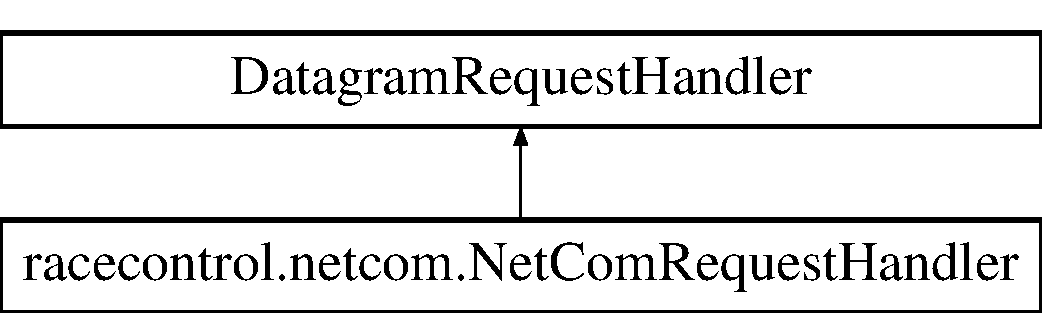
\includegraphics[height=2.000000cm]{classracecontrol_1_1netcom_1_1NetComRequestHandler}
\end{center}
\end{figure}
\subsection*{Public Member Functions}
\begin{DoxyCompactItemize}
\item 
def {\bf handle} (self)
\end{DoxyCompactItemize}


\subsection{Detailed Description}
\begin{DoxyVerb}Inherits from socketserver.DatagramRequestHandler to handle UDP
requests.

For further information, read the handle() methods documentation or the
Python library documentation for socketserver.
\end{DoxyVerb}
 

\subsection{Member Function Documentation}
\index{racecontrol\+::netcom\+::\+Net\+Com\+Request\+Handler@{racecontrol\+::netcom\+::\+Net\+Com\+Request\+Handler}!handle@{handle}}
\index{handle@{handle}!racecontrol\+::netcom\+::\+Net\+Com\+Request\+Handler@{racecontrol\+::netcom\+::\+Net\+Com\+Request\+Handler}}
\subsubsection[{handle(self)}]{\setlength{\rightskip}{0pt plus 5cm}def racecontrol.\+netcom.\+Net\+Com\+Request\+Handler.\+handle (
\begin{DoxyParamCaption}
\item[{}]{self}
\end{DoxyParamCaption}
)}\label{classracecontrol_1_1netcom_1_1NetComRequestHandler_a78fc260655402d03147362ba756f885e}
\begin{DoxyVerb}This method reimplements the handle() method from
socketserver.DatagramRequestHandler. It reads the incoming message.
Through its own sender variable, it accesses the NetCom object
associated with its UDP server object and checks if the source of the
received message is in the node registry. If so, the timestamp for the
node is reset and the message is filtered for protocol words, then
passed to the NetCom object's notify() method. If not, the message is
checked for protocol words. In case this check is successful, the
source IP is passed to the NetCom object's add_node() method to
register it and an appropriate response is generated and sent back to
the source.
\end{DoxyVerb}
 

The documentation for this class was generated from the following file\+:\begin{DoxyCompactItemize}
\item 
racecontrol/netcom.\+py\end{DoxyCompactItemize}

\section{racecontrol.\+netcom.\+Net\+Com\+Server Class Reference}
\label{classracecontrol_1_1netcom_1_1NetComServer}\index{racecontrol.\+netcom.\+Net\+Com\+Server@{racecontrol.\+netcom.\+Net\+Com\+Server}}
Inheritance diagram for racecontrol.\+netcom.\+Net\+Com\+Server\+:\begin{figure}[H]
\begin{center}
\leavevmode
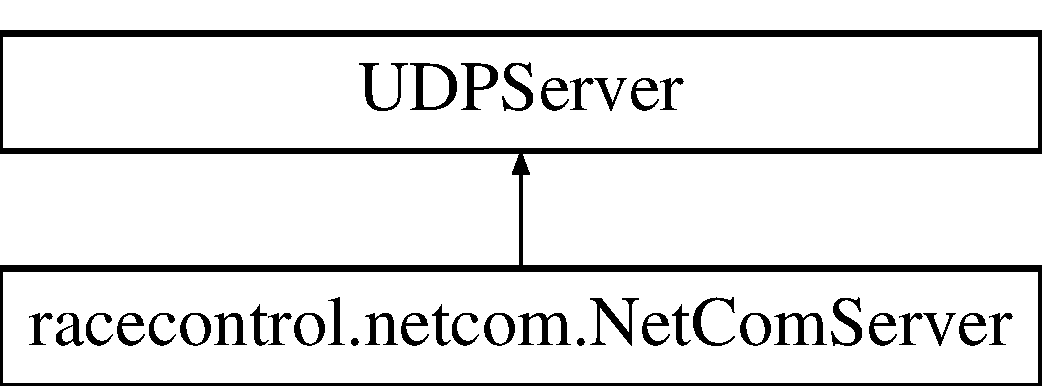
\includegraphics[height=2.000000cm]{classracecontrol_1_1netcom_1_1NetComServer}
\end{center}
\end{figure}
\subsection*{Public Member Functions}
\begin{DoxyCompactItemize}
\item 
def {\bfseries \+\_\+\+\_\+init\+\_\+\+\_\+} (self, server\+\_\+address, Net\+Com\+Request\+Handler\+Class, netcom)\label{classracecontrol_1_1netcom_1_1NetComServer_a9bb05aad9d87c4e06b41c06d6226e91e}

\end{DoxyCompactItemize}
\subsection*{Public Attributes}
\begin{DoxyCompactItemize}
\item 
{\bfseries netcom}\label{classracecontrol_1_1netcom_1_1NetComServer_ae4138cdb5ab515c42227886ff80bf88c}

\end{DoxyCompactItemize}


\subsection{Detailed Description}
\begin{DoxyVerb}Inherits the socketserver.UDPServer class.

Addition made to the parent's __init__() method: Stores a reference to an
associated NetCom object. (Should be a weak reference to not confuse the
garbage collector but currently isn't.)
\end{DoxyVerb}
 

The documentation for this class was generated from the following file\+:\begin{DoxyCompactItemize}
\item 
racecontrol/netcom.\+py\end{DoxyCompactItemize}

\hypertarget{classracecontrol_1_1netcom_1_1Node}{}\section{racecontrol.\+netcom.\+Node Class Reference}
\label{classracecontrol_1_1netcom_1_1Node}\index{racecontrol.\+netcom.\+Node@{racecontrol.\+netcom.\+Node}}
\subsection*{Public Member Functions}
\begin{DoxyCompactItemize}
\item 
def {\bfseries \+\_\+\+\_\+init\+\_\+\+\_\+} (self, ip, last\+\_\+msg=None)\hypertarget{classracecontrol_1_1netcom_1_1Node_ab4657c078f6072dd8c969deb02fc38b4}{}\label{classracecontrol_1_1netcom_1_1Node_ab4657c078f6072dd8c969deb02fc38b4}

\end{DoxyCompactItemize}
\subsection*{Public Attributes}
\begin{DoxyCompactItemize}
\item 
{\bfseries ip}\hypertarget{classracecontrol_1_1netcom_1_1Node_abdff7afa445316fee0d5654d7afb1807}{}\label{classracecontrol_1_1netcom_1_1Node_abdff7afa445316fee0d5654d7afb1807}

\item 
{\bfseries last\+\_\+msg}\hypertarget{classracecontrol_1_1netcom_1_1Node_a94713033f5b908feedd0c8916983e3b5}{}\label{classracecontrol_1_1netcom_1_1Node_a94713033f5b908feedd0c8916983e3b5}

\item 
{\bfseries timestamp}\hypertarget{classracecontrol_1_1netcom_1_1Node_a5c936ec6a989b43b28b349adbca9225e}{}\label{classracecontrol_1_1netcom_1_1Node_a5c936ec6a989b43b28b349adbca9225e}

\end{DoxyCompactItemize}


\subsection{Detailed Description}
\begin{DoxyVerb}Holds node data for all network communication partners.

The Node class holds every communication partner's ip, the last message
received from the partner and the time of reception.
\end{DoxyVerb}
 

The documentation for this class was generated from the following file\+:\begin{DoxyCompactItemize}
\item 
racecontrol/netcom.\+py\end{DoxyCompactItemize}

%--- End generated contents ---

% Index
\backmatter
\newpage
\phantomsection
\clearemptydoublepage
\addcontentsline{toc}{chapter}{Index}
\printindex

\end{document}
